
\section{Ejercicio 2.}

\subsection{Parte a.}

\par Exploramos diferentes layouts para visualizar la red delfines.
En la figura \ref{fig:Layout_delfines} observamos el resultado de graficar
el grafo con el Fruchterman - Reingold layout. 
\par El algoritmo para realizar este layout se basa en asignarles fuerzas de interacción ficticias a los nodos. Típicamente se basa en que los nodos ligados tengan una fuerza de atracción análoga a la fuerza de un resorte, sumado a una fuerza de repulsión entre todos los nodos, análoga a la interacción coloumbiana entre partículas cargadas idénticamente.
\par Este tipo de layout nos permitió visualizar la existencia de dos comunas de delfines, ligadas a través de unos pocos nodos.

\begin{figure}[h]
\centering
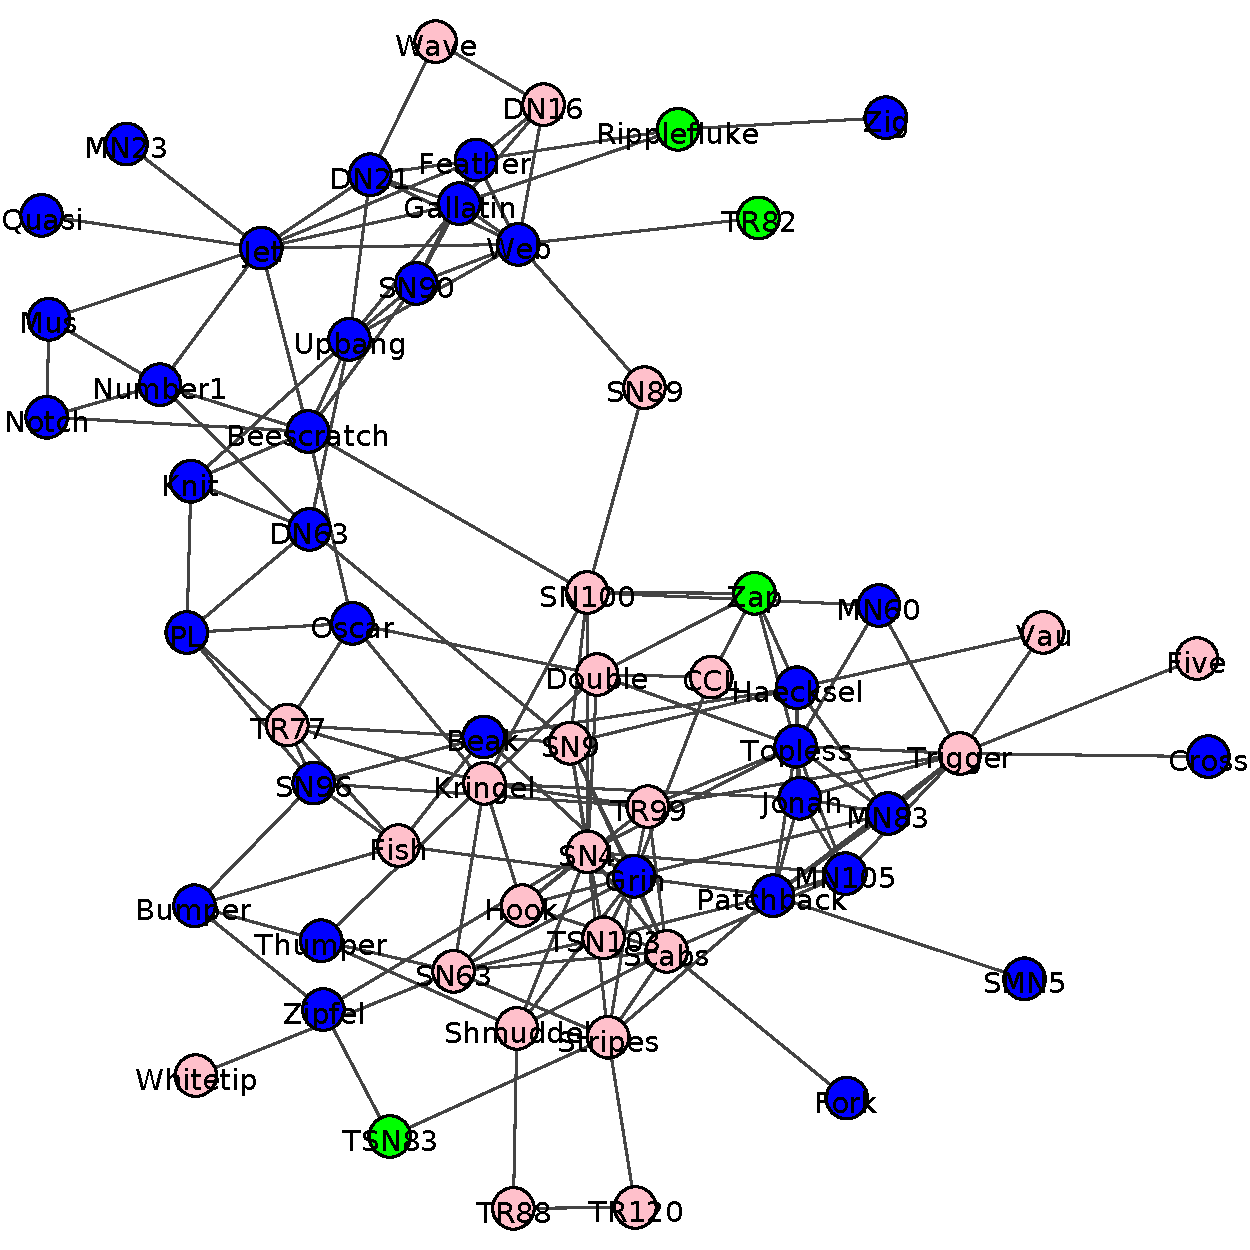
\includegraphics[scale = 0.50]{figuras/FrutRein}
\label{fig:Layout_delfines}
\caption{Fruchterman - Reingold layout. Los colores de los nodos se refieren al sexo del delfín: azul, macho; rosa, hembra; verde, sexo no indicado en el dataset.}
\end{figure}
